\documentclass[12pt]{article}
\usepackage[T2A]{fontenc}
\usepackage[utf8]{inputenc}
\usepackage[russian]{babel}
\usepackage{amsmath, graphicx, float, hyperref}

\graphicspath{{./pictures/}}

\begin{document}
    \begin{titlepage}
        \begin{center}
            \vspace*{1cm}

            \Huge
            \textbf{Закон всемирного тяготения.\\Точки Лагранжа}

            \vspace{1.5cm}

            \Large
            \textbf{Балдин Виктор Б01-303}

            \vfill

            Вопрос по выбору \\
            Устный экзамен по общей физике

            \vspace{0.8cm}

            
\includegraphics[width=0.4\textwidth]{university_logo.png}

            Физтех-школа радиотехники и компьютерных технологий\\
            Московский физико-технический институт\\
            Долгопрудный, 2024
        \end{center}
    \end{titlepage}

    \begin{abstract}
        \par Данный вопрос по выбору включает в себя теоретические расчеты
        положения точек Лагранжа и обсуждение некоторых их интересных
        свойств. В работе используются материалы из различных открытых
        источников об истории исследований на эту тему и современном их
        состоянии.
        \par Точки Лагранжа являются крайне важным объектом для изучения
        космического пространства в современной астрофизике.
        В частности, прямым образом их свойства используются для размещения
        космических аппаратов, предназначенных для наблюдений дальнего
        космоса.
        \par Автор выражает надежду, что данная работа содержит
        актуальные сведения и благодарит экзаменационную комиссию за ее
        рассмотрение.
    \end{abstract}

    \newpage

    \section{Введение}
    \par \textit{Точки Лагранжа}, в некоторых источниках также \textit{точки
    либрации} или \textit{$L$-точки} -- точки в системе двух тел, в которых
    третье тело может оставаться неподвижным относительно первых двух.
    \par Точки Лагранжа названы в честь математика Жозефа Луи Лагранжа,
    который первым в 1772 году показал их существование.

    \begin{figure}[H]
        \centering
        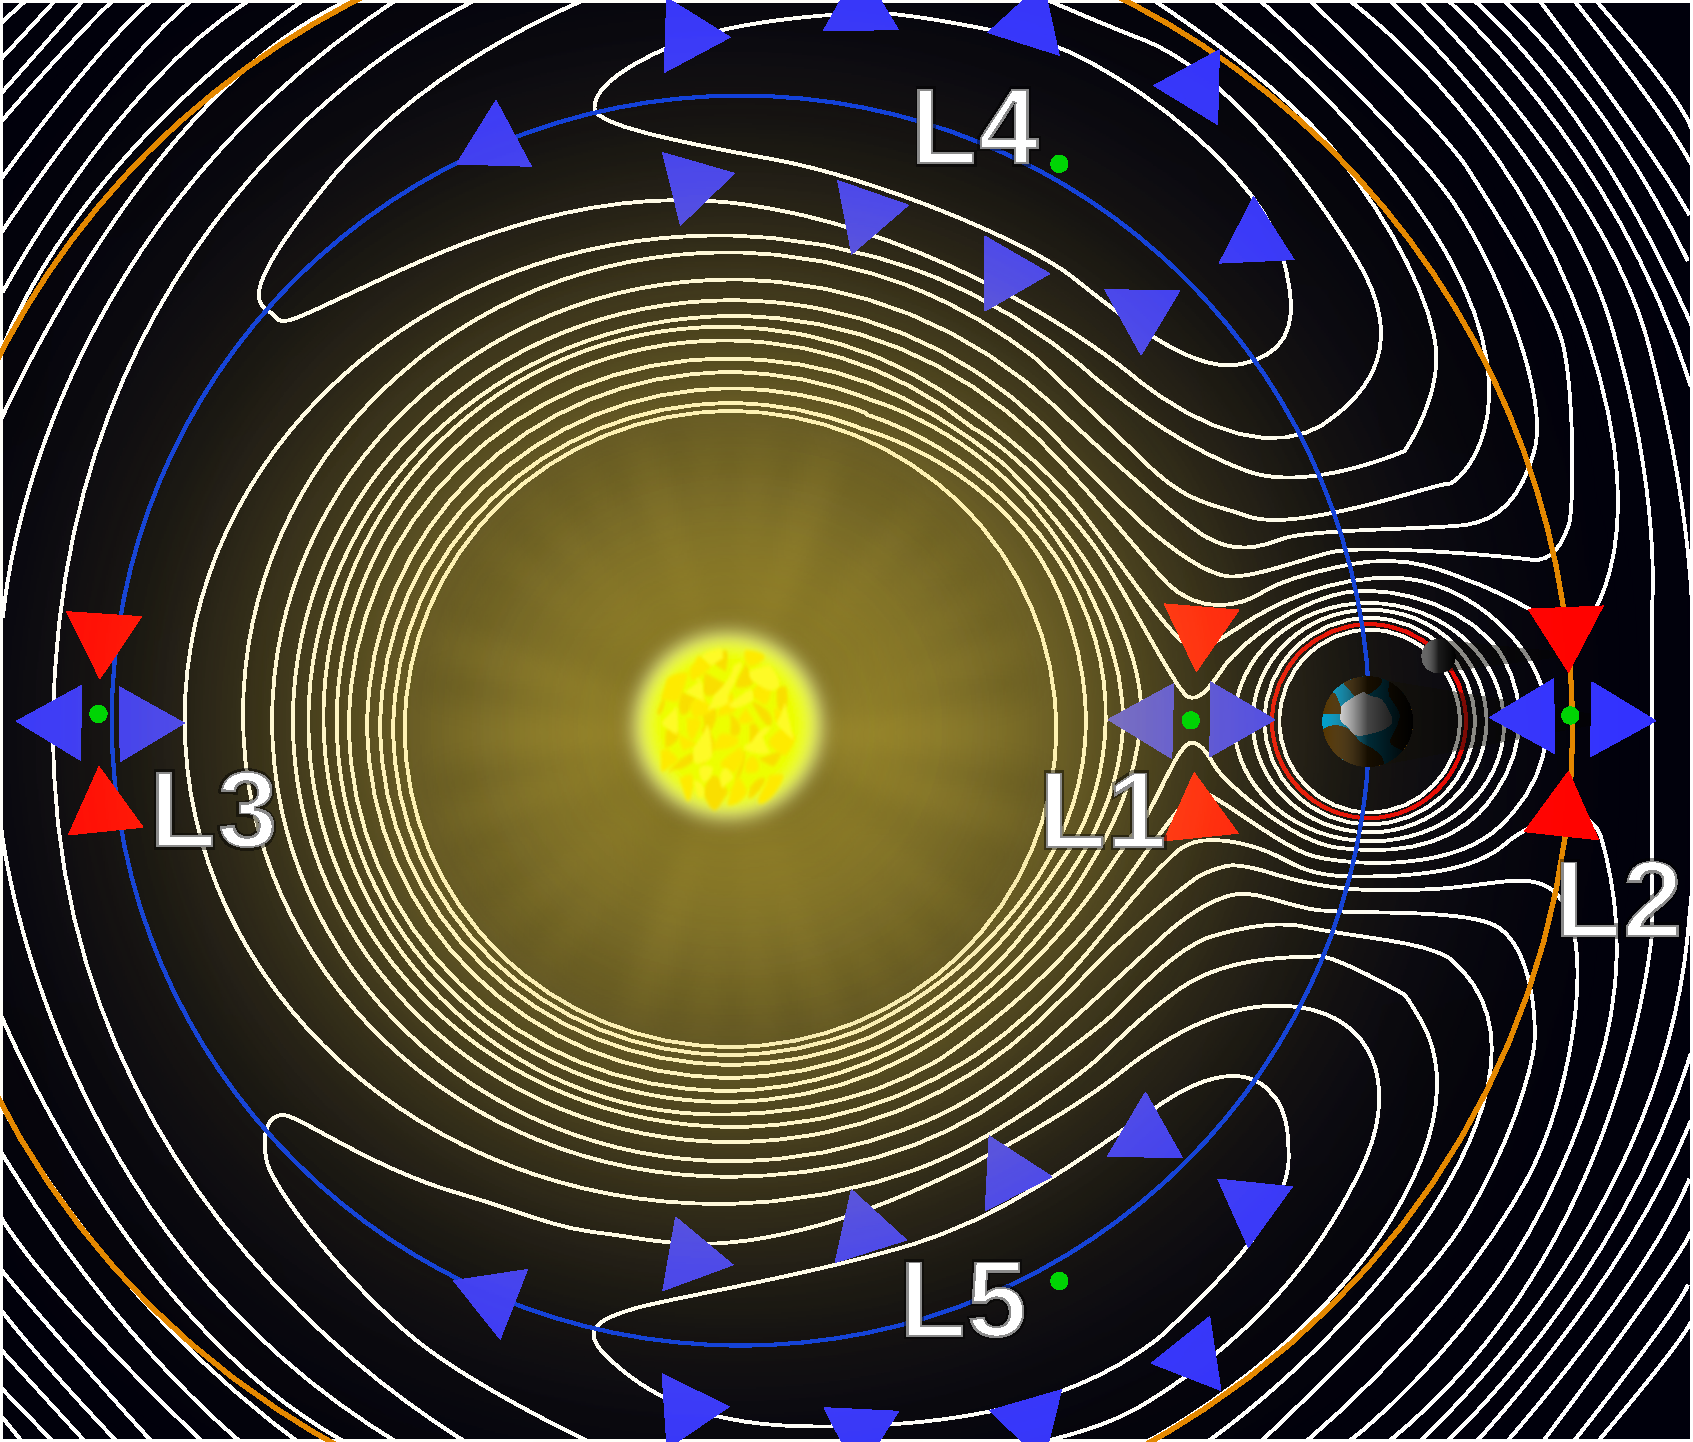
\includegraphics[scale=0.35]{Lagrange_points.pdf}
        \caption{5 точек Лагранжа и гравитационные эквипотенциальные
        поверхности системы двух тел\\
        \textit{Источник:}
        \url{https://upload.wikimedia.org/wikipedia/commons/thumb/e/ee/
        Lagrange_points2.svg/1920px-Lagrange_points2.svg.png}}
    \end{figure}

    \section{Точки Лагранжа}
    \par Для начала проведем краткое рассмотрение движения 3-х тел, связанных между
    собой гравитационными взаимодействиями. Это может быть описано в общем
    случае следующими дифференциальными уравнениями:

    \begin{equation}
        \begin{cases}
            \ddot{\vec{r_1}} = -Gm_2\frac{\vec{r_1} - \vec{r_2}}
            {\lvert \vec{r_1} - \vec{r_2} \rvert} -
            Gm_3\frac{\vec{r_1} - \vec{r_3}}{\lvert \vec{r_1} - 
            \vec{r_3} \rvert}\\
            \ddot{\vec{r_2}} = -Gm_2\frac{\vec{r_2} - \vec{r_3}}
            {\lvert \vec{r_2} - \vec{r_3} \rvert} -
            Gm_3\frac{\vec{r_2} - \vec{r_1}}{\lvert \vec{r_2} - 
            \vec{r_1} \rvert}\\
            \ddot{\vec{r_3}} = -Gm_2\frac{\vec{r_3} - \vec{r_1}}
            {\lvert \vec{r_3} - \vec{r_1} \rvert} -
            Gm_3\frac{\vec{r_3} - \vec{r_2}}{\lvert \vec{r_3} - 
            \vec{r_2} \rvert}\\
        \end{cases}\,.
    \end{equation}

    Данная система имеет множество сложных решений, на которых мы не будем
    останавливаться. В нашу задачу входит частный случай задачи трех тел 
    (англ. \textit{restricted three-body problem}), в котором имеем
    2 массивных тела массами $M_1$ и $M_2$ и третье тело массой $m$, 
    $m \ll M_1$, $m \ll M_2$. В таком случае мы можем рассматривать движение
    $M_1$ и $M_2$ в рамках задачи двух тел, пренебрегая гравитационным
    воздействием третьего тела.
    \par Как известно, два тела в отсутствии внешних гравитационных воздейстсвий
    вращаются относительно центра масс системы. Поэтому теперь мы можем
    поставить задачу конкретнее: найти все возможные положения третьего тела,
    при которых оно будет совершать вращение вокруг центра масс с той же угловой
    скоростью, что и $M_1$ и $M_2$. Логично ввести систему координат с началом в
    центре масс системы. Обозначим радиус-векторы $M_1$ и $M_2$ через $\vec{r_1}$
    и $\vec{r_2}$ соответственно.

    \begin{figure}[H]
        \centering
        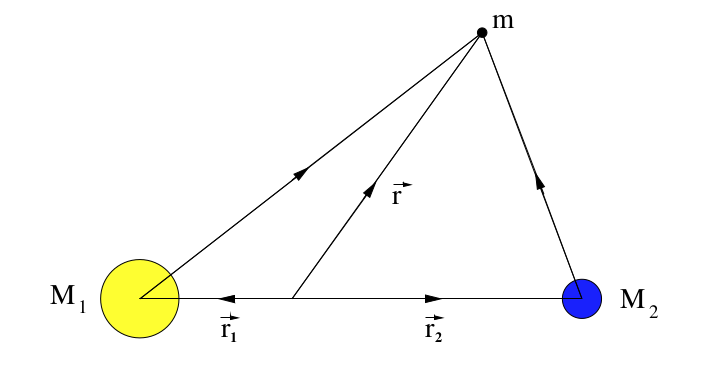
\includegraphics[scale = 2]{two-bodies.png}
        \caption{Рассматриваемый частный случай задачи трех тел}
    \end{figure}

    Понятно, что теперь мы можем написать уравнение для ускорения тела $m$, 
    исходя из закона всемирного тяготения:
    
    \begin{equation}
        \ddot{\vec{r}} = -\frac{GM_1}{\lvert \vec{r} - \vec{r_1} \rvert^3}
        (\vec{r} - \vec{r_1}) - \frac{GM_2}{\lvert \vec{r} - \vec{r_2} \rvert^3}
        (\vec{r} - \vec{r_2}) 
    \end{equation}

    \par Теперь из третьего закона Кеплера найдем угловую скорость вращения системы
    $M_1$ и $M_2$:

    \begin{equation}
        \Omega^2 R^3 = G(M_1 + M_2), 
    \end{equation}

    где $R$ -- расстояние между телами. 

    \par
    Введем обозначения:
    $$ \alpha = \frac{M_2}{M_1 + M_2}, \beta = \frac{M_1}{M_1 + M_2} $$

    \par Для дальнейших рассуждений полезно ввести прямоугольный ортонормированный
    базис: $\vec{k} = \frac{\vec{\Omega}}{\lvert \vec{\Omega} \rvert}$, 
    $\vec{i} = \frac{\vec{r_2}}{\lvert \vec{r_2} \rvert}$, $\vec{j} =
    [ \vec{k}, \vec{i} ]$. В этом базисе:

    \begin{eqnarray*}
        \vec{r}   = x(t)\vec{i} + y(t)\vec{j}\\
        \vec{r_1} = -\alpha R\vec{i}\\
        \vec{r_2} = \beta R\vec{i}
    \end{eqnarray*}

    \begin{thebibliography}{10}
        \bibitem{sivukhin}
        Д. В. Сивухин (2005) \emph{Общий курс физики. Том 1: Механика}
        
        \bibitem{enwikipedia}
        \url{https://en.wikipedia.org/wiki/Lagrange_point}

        \bibitem{mit18}
        \url{https://ocw.mit.edu/courses/16-07-dynamics-fall-2009/resources/mit16_07f09_lec18/}

        \bibitem{nasa}
        \url{https://wmap.gsfc.nasa.gov/media/ContentMedia/lagrange.pdf}
    \end{thebibliography}

\end{document}
